% Source: outputs/polynomial_duration_cutoff_sweep/n100/report.html
% Settings: simulations/configuration.json and baseline_30us/configuration.json.
% Numerical results: metrics_all.csv and comparison_summary.json in that directory.
% Convergence evidence: validation/convergence.json (45 representative traces).
% Contrast tables use saved scan.npz contrast, checked against metrics_all.csv.
% Maximin contrast/FWHM: figures/paper/supp_extended_cutoff_duration_summary.json.
\section{Extended Cutoff and Pulse-Duration Range}
\label{sec:extended-cutoff-duration}

The duration--cutoff comparison in the main text displays the
$10^{-5}\leq c\leq10^{-2}$ portion of a larger numerical survey. Here we
consider the full range, comprising 100 logarithmically spaced cutoffs from
$10^{-5}$ to 1 and pulse durations $L=10$, 20, 30, 45, and
$60~\mu\mathrm{s}$. For every pair $(L,c)$, we simulate 100 nominal drive
scales $\Omega_0/(2\pi)$ from 0 to $100~\mathrm{MHz}$ and 201 detunings
$\Delta/(2\pi)$ from $-0.5$ to $0.5~\mathrm{MHz}$. This survey contains
50\,000 spectra and 10\,050\,000 simulated operating points. It extends the
parameter range of the three-level calculation, rather than the range of
experimental validation. Figure~\ref{fig:extended-cutoff-duration} displays
the full cutoff--drive maps for all five pulse lengths, with common color
scales for linewidth and visibility.

\subsection{Pulse family and comparison metrics}

We use the polynomial-corrected DRAG echo introduced in
Sec.~\ref{sec:pulse-modifications}. The unsigned envelope is the
cutoff-subtracted root-Lorentzian multiplied
by the fixed polynomial window,
\begin{equation}
    \begin{gathered}
    g(t)=\frac{[1+(t/\sigma)^2]^{-1/2}-c}{1-c}
    \left[1-\left(\frac{2t}{L}\right)^2\right]^5,
    \\
    \sigma=\frac{L}{2}\frac{c}{\sqrt{1-c^2}},
    \end{gathered}
    \label{eq:extended-cutoff-envelope}
\end{equation}
for $|t|<L/2$, with zero drive outside. The signed drive is
$I(t)=\Omega_0g(t)s(t)$, where $s(t)$ reverses sign through the same
$16~\mathrm{ns}$ sine transition at every operating point. The complex
drive is $I-iQ$, with $Q=-\beta\dot I/|\alpha|$ and $\beta=-0.5$;
$\alpha$ is an angular frequency and the derivative includes both $g$ and
$s$. The unsigned midpoint normalization is fixed, without pulse-area or
smoothed-peak renormalization. The three-level Lindblad model uses
$\alpha/(2\pi)=-216~\mathrm{MHz}$, $T_1=51.24~\mu\mathrm{s}$, and
$T_2=7.31~\mu\mathrm{s}$, with no added phenomenological Stark correction.

For this corrected pulse, $c$ specifies the original root-Lorentzian core
width; the actual endpoint amplitude vanishes for every cutoff. Thus the
endpoint-jump estimate in Sec.~\ref{sec:pulse-cutoff} does not directly
describe this family. Increasing $L$ at fixed $c$ also broadens $\sigma$,
so this is not a sweep of tail duration at fixed core width. Moreover,
the apparently singular endpoint $c=1$ has the continuous limit
\begin{equation}
    g(t)\big|_{c=1}=
    \left[1-\left(\frac{2t}{L}\right)^2\right]^6.
    \label{eq:extended-cutoff-one-limit}
\end{equation}
It is therefore a smooth polynomial envelope, not a square pulse.

We extract a local dip FWHM $\Gamma_f$ after subtracting a linear background
fitted over $0.4\leq|\Delta/(2\pi)|\leq0.5~\mathrm{MHz}$. The dip-center
search is restricted to $\pm0.25~\mathrm{MHz}$, and the width uses the
nearest half-depth crossings. Widths spanning fewer than six detuning
intervals ($30~\mathrm{kHz}$) are rejected, as are unresolved dips and
nonpositive shoulder contrast. Additional minima with population prominence
at least 0.005 are counted but do not automatically invalidate a local width.
Acceptance consequently does not certify a unique resonance.

Contrast is the height of a peak or depth of a dip relative to its local
background, expressed as a probability difference on a scale from 0 to 1.
For the simulated dips we use the same background as the FWHM extraction,
\begin{equation}
    C=P_{\mathrm{bg}}(\delta_*)-P_e(\delta_*),
    \qquad \delta=\Delta/(2\pi),
    \label{eq:extended-cutoff-contrast}
\end{equation}
where $\delta_*$ is the sampled detuning of maximum background-relative
depth within the central search interval. For a peak, the sign is reversed.
A contrast of $0.3$ therefore means a difference of 0.3 in excitation
probability. Contrast is not divided by a noise estimate and is independent
of the assumed number of shots. The reference
$\Gamma_{f,T_2}=1/(\pi T_2)=43.5~\mathrm{kHz}$ provides a common linewidth
scale, not an assertion that these shaped pulses attain that limit.

\begin{figure*}[!tp]
    \centering
    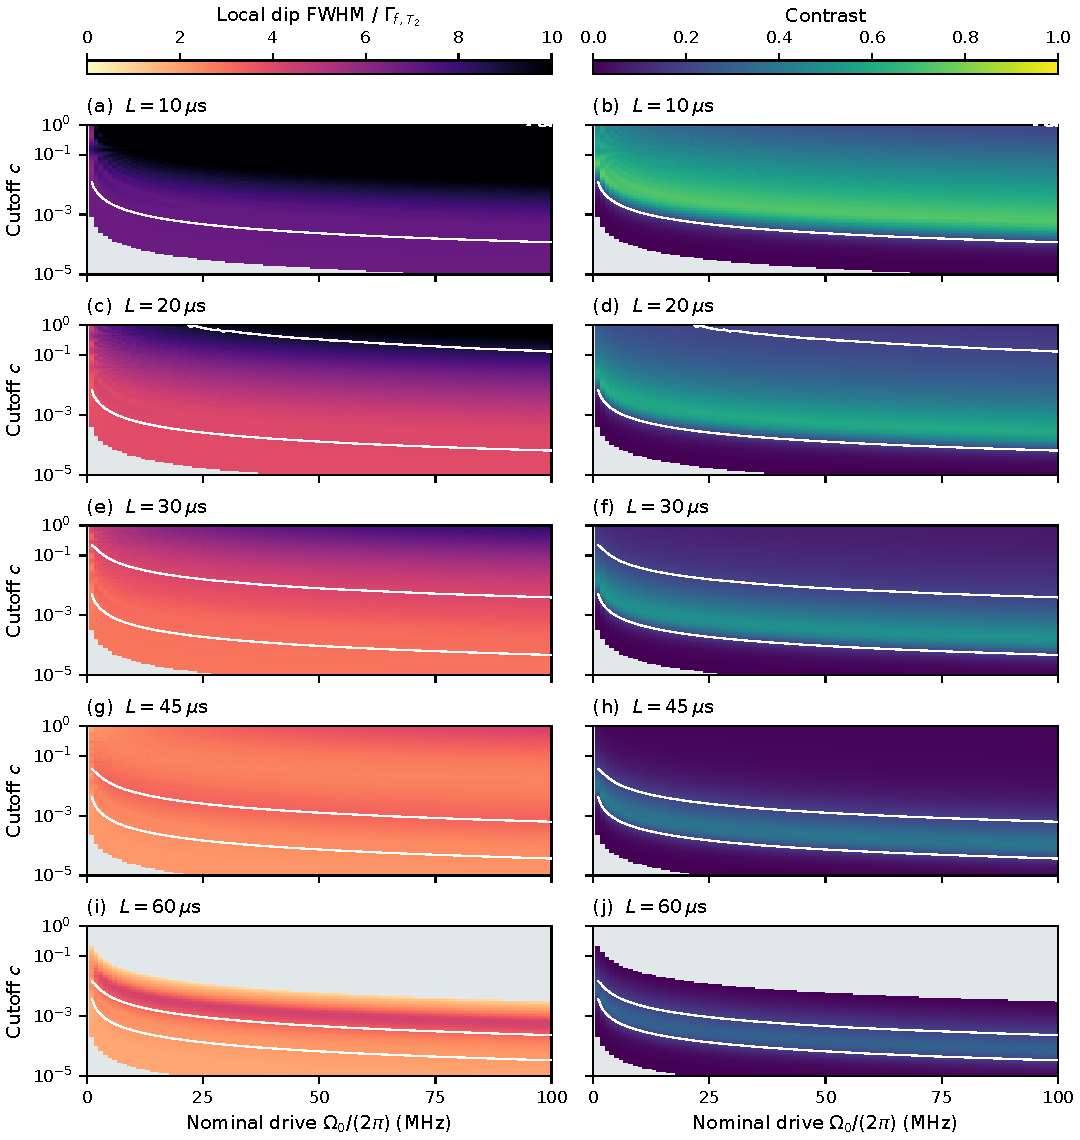
\includegraphics[width=\textwidth]{../figures/paper/supp_extended_cutoff_duration.pdf}
    \caption{Full cutoff--duration survey for the polynomial-corrected DRAG
    echo. Rows show $L=10$, 20, 30, 45, and $60~\mu\mathrm{s}$.
    Left: dip FWHM divided by $\Gamma_{f,T_2}=43.5~\mathrm{kHz}$;
    lighter colors indicate narrower linewidths, and values above 10
    saturate at the darkest color. Right: probability contrast
    $C$ [Eq.~\eqref{eq:extended-cutoff-contrast}]. Thin white contours in both
    columns mark $C=0.2$, interpolated between accepted samples. Each panel contains
    100 logarithmic cutoffs and 100 drive scales spanning the displayed axes.
    Color scales are shared across rows; gray cells are rejected dips.
    All pulses use $p=5$, $\beta=-0.5$, and a $16~\mathrm{ns}$ sine
    inversion. Heatmaps show saved cells without interpolation.}
    \label{fig:extended-cutoff-duration}
\end{figure*}

\subsection{Large-cutoff behavior and the duration tradeoff}

The extended range shows why neither minimizing cutoff nor increasing it
toward unity is sufficient to obtain useful resolution.
Table~\ref{tab:extended-cutoff-examples} gives representative sampled
cutoffs for $L=30~\mu\mathrm{s}$ at
$\Omega_0/(2\pi)=49.495~\mathrm{MHz}$. The smallest cutoff gives a narrower
accepted dip but contrast of only $0.0027$. Around $c=10^{-3}$ the signal is much
stronger; extending toward $c\simeq0.1$ and 1 broadens the local feature
while reducing its contrast. This high-cutoff degradation occurs despite zero
endpoint amplitude and must be distinguished from abrupt-truncation artifacts.

\begin{table}[!tp]
    \caption{Representative points from the extended cutoff sweep at
    $L=30~\mu\mathrm{s}$ and $\Omega_0/(2\pi)=49.495~\mathrm{MHz}$.
    Cutoffs are rounded saved samples; all listed widths pass the local-dip
    screen. Contrast follows Eq.~\eqref{eq:extended-cutoff-contrast}.}
    \label{tab:extended-cutoff-examples}
    \begin{ruledtabular}
    \begin{tabular}{ccc}
        Cutoff $c$ & FWHM (kHz) & Contrast $C$ \\
        $10^{-5}$             & 125.7 & 0.0027 \\
        $1.048\times10^{-3}$  & 150.4 & 0.3878 \\
        $9.545\times10^{-3}$  & 181.9 & 0.1895 \\
        $9.770\times10^{-2}$  & 237.9 & 0.1093 \\
        $1$                   & 325.9 & 0.0782
    \end{tabular}
    \end{ruledtabular}
\end{table}

Duration changes this balance. At the same drive and
$c=1.048\times10^{-3}$, increasing $L$ from 10 to $45~\mu\mathrm{s}$
reduces FWHM from 308.6 to $138.9~\mathrm{kHz}$ while contrast falls from
0.723 to 0.220. At $60~\mu\mathrm{s}$, the width rises to
$187.5~\mathrm{kHz}$ and contrast falls to 0.114. At large cutoff, a narrower
local feature can instead accompany nearly lost visibility: for
$L=45~\mu\mathrm{s}$ and $c=1$, FWHM is $166.1~\mathrm{kHz}$ but contrast
is only 0.0117; the corresponding $60~\mu\mathrm{s}$ spectrum fails the
local-dip screen. These examples show that linewidth alone does not quantify
usable sensitivity, and the duration dependence is not a universal $1/L$
narrowing law.

\subsection{One cutoff across the drive range}

To quantify robustness without retuning cutoff at each drive, we select one
cutoff per duration by maximizing the minimum $C/\Gamma_f$
over all 90 sampled drive scales from 10.101 to $100~\mathrm{MHz}$.
A candidate must have an accepted dip at every one of these scales.
Table~\ref{tab:extended-cutoff-robustness} reports the sampled selections;
the worst width and minimum contrast need not occur at the same drive.

\begin{table}[!tp]
    \caption{Fixed-cutoff selections maximizing the worst sampled
    contrast/FWHM over the drive range. These are discrete survey results,
    without interpolation or a continuous optimization. Width and contrast
    extrema are evaluated separately at the selected cutoff.}
    \label{tab:extended-cutoff-robustness}
    \begin{ruledtabular}
    \setlength{\tabcolsep}{4pt}
    \begin{tabular}{@{}ccccc@{}}
        \shortstack{$L$\\($\mu$s)} & Cutoff $c$
        & \shortstack{Max. FWHM\\(kHz)} & Min. $C$
        & \shortstack{Min. $C/\Gamma_f$\\(MHz$^{-1}$)} \\
        10 & $2.656\times10^{-3}$ & 362.5 & 0.574 & 1.740 \\
        20 & $1.177\times10^{-3}$ & 205.1 & 0.452 & 2.270 \\
        30 & $6.579\times10^{-4}$ & 154.9 & 0.321 & 2.329 \\
        45 & $3.678\times10^{-4}$ & 133.2 & 0.202 & 1.944 \\
        60 & $2.310\times10^{-4}$ & 145.4 & 0.123 & 1.371
    \end{tabular}
    \end{ruledtabular}
\end{table}

The selected cutoff decreases with duration. The 20 and $30~\mu\mathrm{s}$
pulses have similar worst-case contrast/FWHM, with the latter trading some signal
for a smaller worst-case width. The selected 10, 20, and $30~\mu\mathrm{s}$
pulses maintain contrast above 0.3 throughout the sampled drive interval;
the selected 45 and $60~\mu\mathrm{s}$ pulses have minimum contrasts of
0.202 and 0.123, respectively. Even the smallest
worst-case widths in this comparison remain about three times the
$T_2$ reference linewidth. Contrast/FWHM is a heuristic tradeoff score rather
than a frequency-estimation uncertainty. These selections do not establish
a global waveform optimum or an experimentally calibrated operating point.

\subsection{Numerical resolution and scope}

The integration uses fourth-order Runge--Kutta propagation with a maximum
time step of $0.25~\mathrm{ns}$ and local refinement near the core and
midpoint transition. Representative convergence checks cover all five
durations at $c=10^{-5}$, $1.048\times10^{-3}$, and 1, and nominal
drives of 10.101, 49.495, and $100~\mathrm{MHz}$ (45 spectra).
Halving the time step changes populations by at most $1.28\times10^{-4}$ and
accepted FWHM by $0.254~\mathrm{kHz}$.
Doubling the detuning intervals changes accepted FWHM by at most
$0.116~\mathrm{kHz}$. Neither refinement changes dip
acceptance in these checks. Metric differences include only spectra accepted
at both resolutions. These checks support the representative comparisons,
including the $c=1$ limit, but are not a full-grid error bound. The fixed
detuning window and background convention also limit the interpretation of
broad or structured spectra, independently of integration accuracy.

